\documentclass[border=10pt]{standalone}
\usepackage{tikz}
\usepackage{xcolor}
\usepackage{booktabs}
\usepackage{dirtree}
\usepackage{array}
\usepackage{helvet}
\renewcommand{\familydefault}{\sfdefault}
\usetikzlibrary{positioning,arrows.meta,shapes,backgrounds,fit,calc}

% Color definitions
\definecolor{treebg}{HTML}{F5F5F5}
\definecolor{boxbg}{HTML}{FFFFFF}
\definecolor{boxborder}{HTML}{CCCCCC}
\definecolor{highlight}{HTML}{FFF9E6}
\definecolor{darktext}{HTML}{2C3E50}
\definecolor{arrowcol}{HTML}{E74C3C}

\newcommand{\filelabel}[1]{%
  \tikz[]\node[draw=arrowcol,inner sep=0pt,minimum size=0.45cm,font=\bfseries]{#1};%
}

\begin{document}
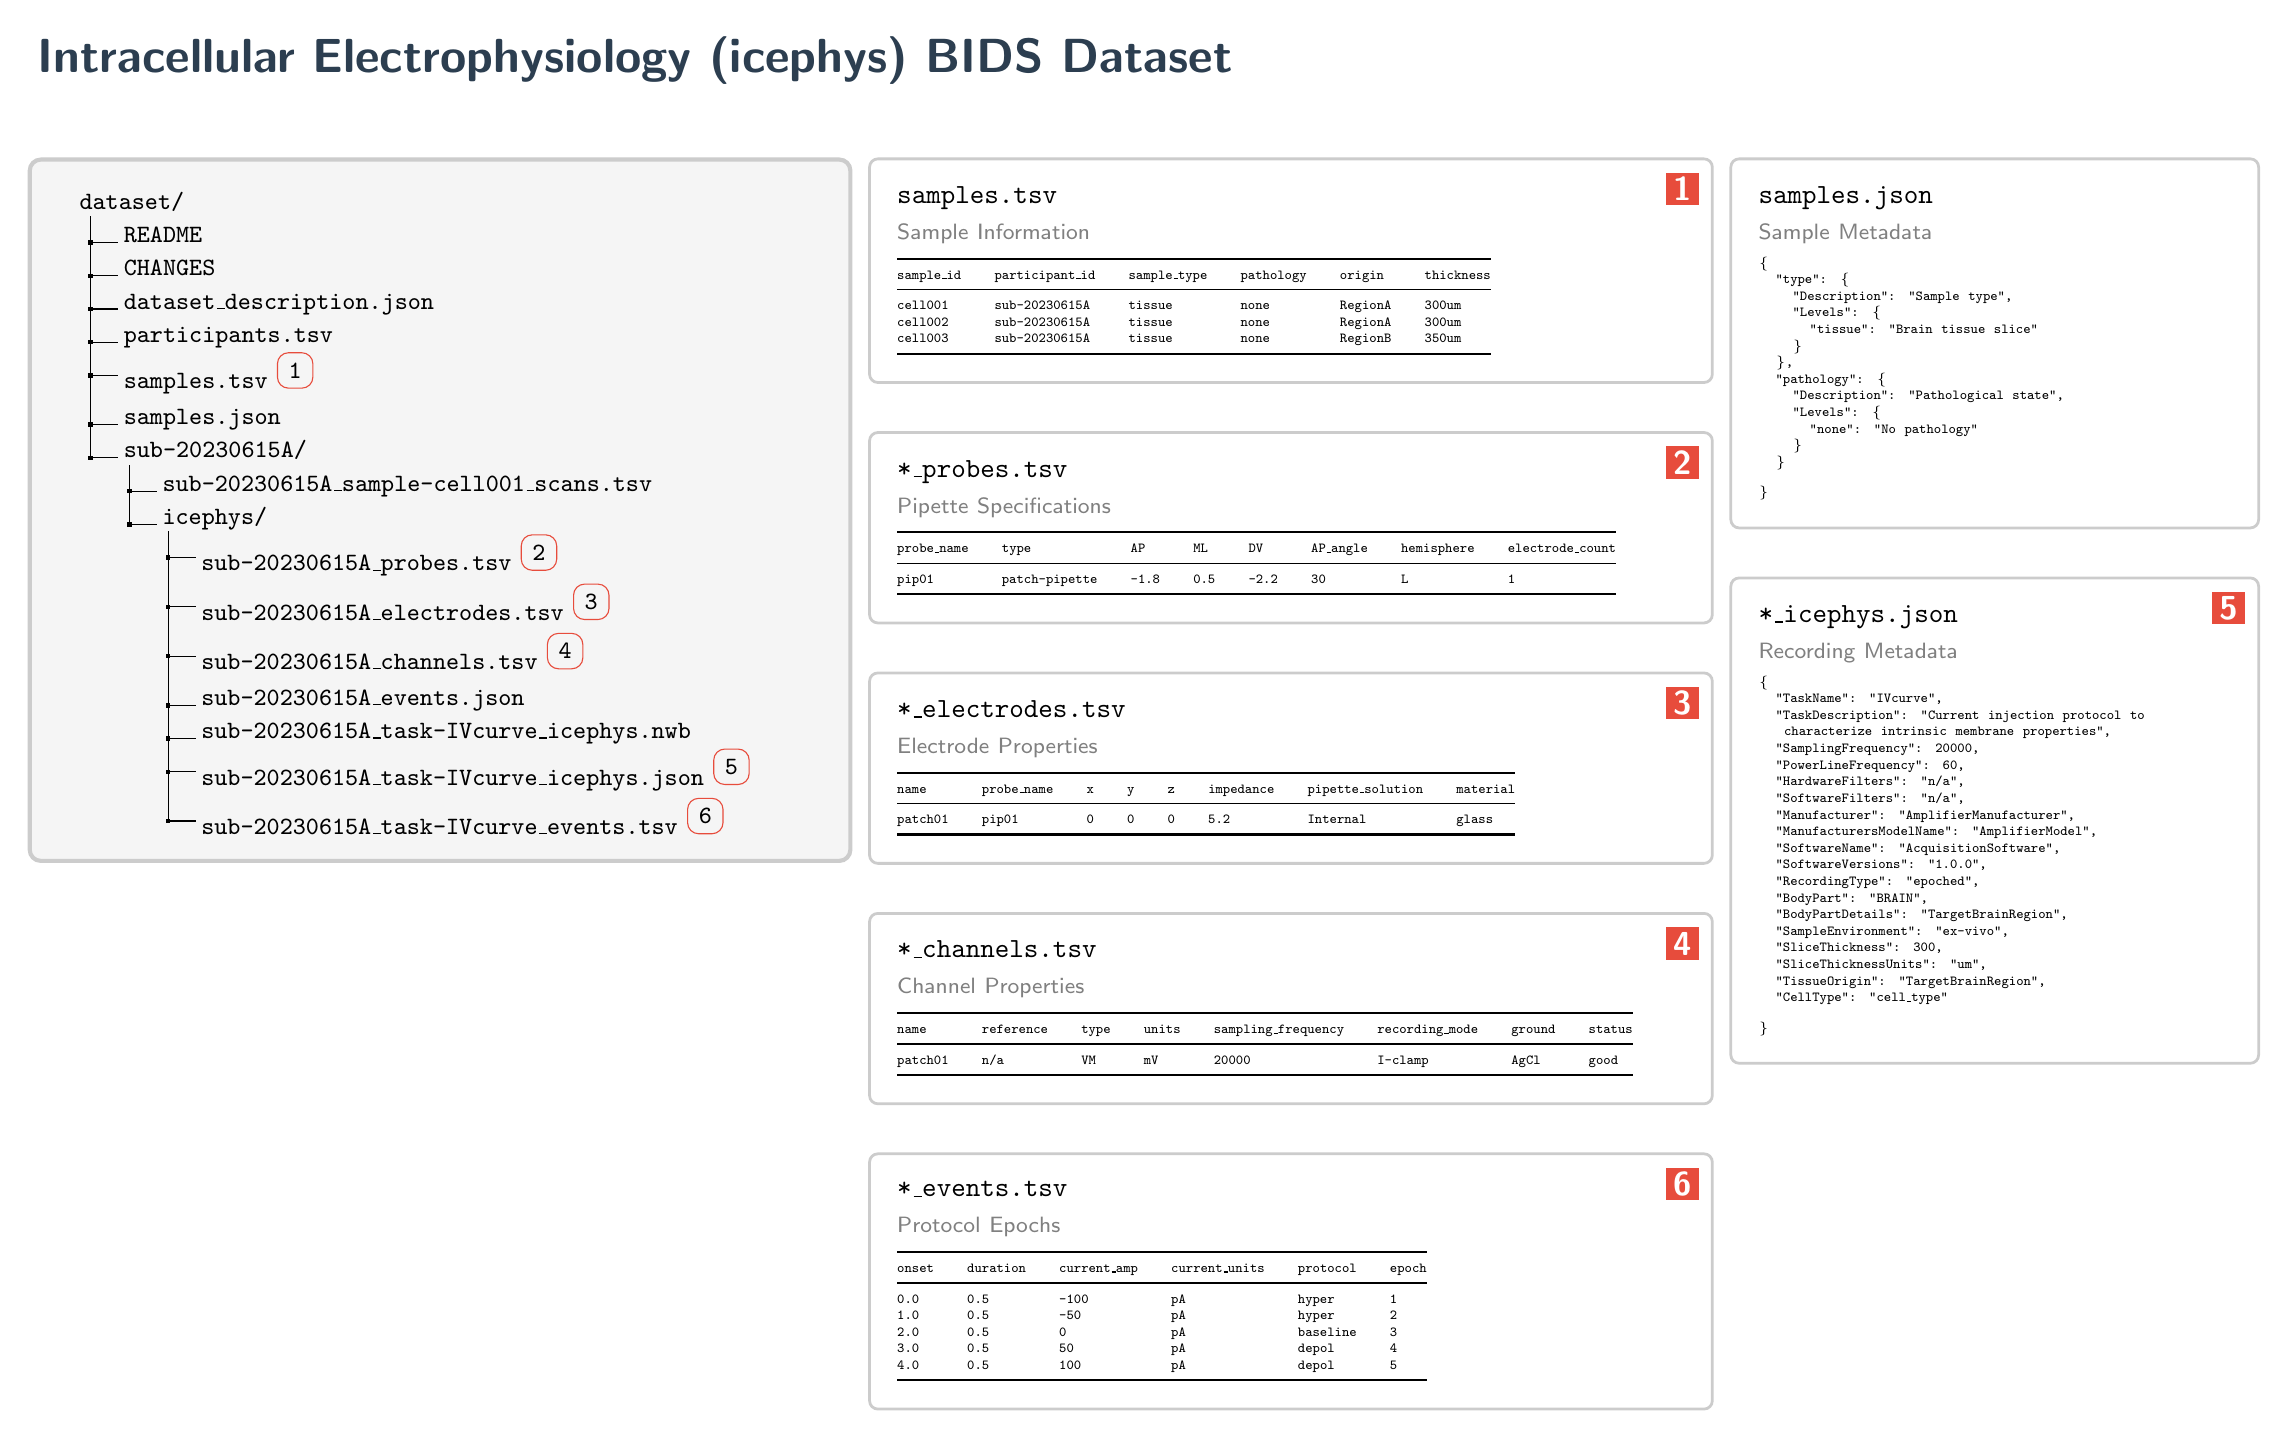
\begin{tikzpicture}[
    node distance=0.4cm,
    contentbox/.style={
        rectangle,
        draw=boxborder,
        fill=boxbg,
        line width=1pt,
        rounded corners=3pt,
        inner sep=10pt,
        text width=8cm,
        align=left,
        font=\small
    },
    widecontentbox/.style={
        rectangle,
        draw=boxborder,
        fill=boxbg,
        line width=1pt,
        rounded corners=3pt,
        inner sep=10pt,
        text width=10cm,
        align=left,
        font=\small
    },
    narrowcontentbox/.style={
        rectangle,
        draw=boxborder,
        fill=boxbg,
        line width=1pt,
        rounded corners=3pt,
        inner sep=10pt,
        text width=6cm,
        align=left,
        font=\small
    },
    labelstyle/.style={
        % circle,
        draw=arrowcol,
        fill=arrowcol,
        inner sep=0pt,
        minimum size=0.4cm,
        font=\bfseries\large,
        text=white
    }
]

% Title at top
\node[font=\LARGE\bfseries, text=darktext] (title) {
    Intracellular Electrophysiology (icephys) BIDS Dataset
};

% File tree
\node[below=0.8cm of title.south west, anchor=north west, fill=treebg, draw=boxborder, line width=1.5pt, rounded corners=4pt, inner sep=6pt, text width=10cm] (treenode) {
{\small\ttfamily
\dirtree{%
.1 dataset/.
.2 README.
.2 CHANGES.
.2 dataset\_description.json.
.2 participants.tsv.
.2 samples.tsv \filelabel{1}.
.2 samples.json.
.2 sub-20230615A/.
.3 sub-20230615A\_sample-cell001\_scans.tsv.
.3 icephys/.
.4 sub-20230615A\_probes.tsv \filelabel{2}.
.4 sub-20230615A\_electrodes.tsv \filelabel{3}.
.4 sub-20230615A\_channels.tsv \filelabel{4}.
.4 sub-20230615A\_events.json.
.4 sub-20230615A\_task-IVcurve\_icephys.nwb.
.4 sub-20230615A\_task-IVcurve\_icephys.json \filelabel{5}.
.4 sub-20230615A\_task-IVcurve\_events.tsv \filelabel{6}.
}
}
};

% COLUMN 1 - TSV FILES
% Box 1: samples.tsv
\node[widecontentbox, right=0.2cm of treenode.north east, anchor=north west] (box1) {
    \textbf{\normalsize\ttfamily samples.tsv}\\[2pt]
    {\footnotesize\textcolor{gray}{Sample Information}}\\[4pt]
    {\tiny\ttfamily
    \begin{tabular}{@{}llllll@{}}
    \toprule
    sample\_id & participant\_id & sample\_type & pathology & origin & thickness \\
    \midrule
    cell001 & sub-20230615A & tissue & none & RegionA & 300um \\
    cell002 & sub-20230615A & tissue & none & RegionA & 300um \\
    cell003 & sub-20230615A & tissue & none & RegionB & 350um \\
    \bottomrule
    \end{tabular}
    }
};
\node[labelstyle] at ([xshift=-0.4cm, yshift=-0.4cm]box1.north east) {1};

% Box 2: probes.tsv
\node[widecontentbox, below=0.6cm of box1.south west, anchor=north west] (box2) {
    \textbf{\normalsize\ttfamily *\_probes.tsv}\\[2pt]
    {\footnotesize\textcolor{gray}{Pipette Specifications}}\\[4pt]
    {\tiny\ttfamily
    \begin{tabular}{@{}llllllll@{}}
    \toprule
    probe\_name & type & AP & ML & DV & AP\_angle & hemisphere & electrode\_count \\
    \midrule
    pip01 & patch-pipette & -1.8 & 0.5 & -2.2 & 30 & L & 1 \\
    \bottomrule
    \end{tabular}
    }
};
\node[labelstyle] at ([xshift=-0.4cm, yshift=-0.4cm]box2.north east) {2};

% Box 3: electrodes.tsv
\node[widecontentbox, below=0.6cm of box2.south west, anchor=north west] (box3) {
    \textbf{\normalsize\ttfamily *\_electrodes.tsv}\\[2pt]
    {\footnotesize\textcolor{gray}{Electrode Properties}}\\[4pt]
    {\tiny\ttfamily
    \begin{tabular}{@{}llllllll@{}}
    \toprule
    name & probe\_name & x & y & z & impedance & pipette\_solution & material \\
    \midrule
    patch01 & pip01 & 0 & 0 & 0 & 5.2 & Internal & glass \\
    \bottomrule
    \end{tabular}
    }
};
\node[labelstyle] at ([xshift=-0.4cm, yshift=-0.4cm]box3.north east) {3};

% Box 4: channels.tsv
\node[widecontentbox, below=0.6cm of box3.south west, anchor=north west] (box4) {
    \textbf{\normalsize\ttfamily *\_channels.tsv}\\[2pt]
    {\footnotesize\textcolor{gray}{Channel Properties}}\\[4pt]
    {\tiny\ttfamily
    \begin{tabular}{@{}llllllll@{}}
    \toprule
    name & reference & type & units & sampling\_frequency & recording\_mode & ground & status \\
    \midrule
    patch01 & n/a & VM & mV & 20000 & I-clamp & AgCl & good \\
    \bottomrule
    \end{tabular}
    }
};
\node[labelstyle] at ([xshift=-0.4cm, yshift=-0.4cm]box4.north east) {4};

% Box 6: events.tsv
\node[widecontentbox, below=0.6cm of box4.south west, anchor=north west] (box6) {
    \textbf{\normalsize\ttfamily *\_events.tsv}\\[2pt]
    {\footnotesize\textcolor{gray}{Protocol Epochs}}\\[4pt]
    {\tiny\ttfamily
    \begin{tabular}{@{}llllll@{}}
    \toprule
    onset & duration & current\_amp & current\_units & protocol & epoch \\
    \midrule
    0.0 & 0.5 & -100 & pA & hyper & 1 \\
    1.0 & 0.5 & -50 & pA & hyper & 2 \\
    2.0 & 0.5 & 0 & pA & baseline & 3 \\
    3.0 & 0.5 & 50 & pA & depol & 4 \\
    4.0 & 0.5 & 100 & pA & depol & 5 \\
    \bottomrule
    \end{tabular}
    }
};
\node[labelstyle] at ([xshift=-0.4cm, yshift=-0.4cm]box6.north east) {6};

% COLUMN 2 - JSON FILES
% Box 7: samples.json
\node[narrowcontentbox, right=0.2cm of box1.north east, anchor=north west] (box7) {
    \textbf{\normalsize\ttfamily samples.json}\\[2pt]
    {\footnotesize\textcolor{gray}{Sample Metadata}}\\[4pt]
    {\tiny\ttfamily
    \{\\
    ~~"type": \{\\
    ~~~~"Description": "Sample type",\\
    ~~~~"Levels": \{\\
    ~~~~~~"tissue": "Brain tissue slice"\\
    ~~~~\}\\
    ~~\},\\
    ~~"pathology": \{\\
    ~~~~"Description": "Pathological state",\\
    ~~~~"Levels": \{\\
    ~~~~~~"none": "No pathology"\\
    ~~~~\}\\
    ~~\}\\
    \}
    }
};

% Box 5: icephys.json
\node[narrowcontentbox, below=0.6cm of box7.south west, anchor=north west] (box5) {
    \textbf{\normalsize\ttfamily *\_icephys.json}\\[2pt]
    {\footnotesize\textcolor{gray}{Recording Metadata}}\\[4pt]
    {\tiny\ttfamily
    \{\\
    ~~"TaskName": "IVcurve",\\
    ~~"TaskDescription": "Current injection protocol to\\
    ~~~characterize intrinsic membrane properties",\\
    ~~"SamplingFrequency": 20000,\\
    ~~"PowerLineFrequency": 60,\\
    ~~"HardwareFilters": "n/a",\\
    ~~"SoftwareFilters": "n/a",\\
    ~~"Manufacturer": "AmplifierManufacturer",\\
    ~~"ManufacturersModelName": "AmplifierModel",\\
    ~~"SoftwareName": "AcquisitionSoftware",\\
    ~~"SoftwareVersions": "1.0.0",\\
    ~~"RecordingType": "epoched",\\
    ~~"BodyPart": "BRAIN",\\
    ~~"BodyPartDetails": "TargetBrainRegion",\\
    ~~"SampleEnvironment": "ex-vivo",\\
    ~~"SliceThickness": 300,\\
    ~~"SliceThicknessUnits": "um",\\
    ~~"TissueOrigin": "TargetBrainRegion",\\
    ~~"CellType": "cell\_type"\\
    \}
    }
};
\node[labelstyle] at ([xshift=-0.4cm, yshift=-0.4cm]box5.north east) {5};

% Background
\begin{scope}[on background layer]
\fill[white] (current bounding box.south west) rectangle (current bounding box.north east);
\end{scope}

\end{tikzpicture}
\end{document}
